\section{Conclusion} \label{cha:researchconclusion}
In short, the mirror game seems the best solution to the problem. It is a viable
project to create in the given time frame, it is a challenging puzzle game even
when playing a different version of it (a single-player version) on your own,
and it taxes the communication of both the remote and the local players, as they
both have abilities necessary for achieving the goal, but they cannot achieve it
on their own (although this could be relaxed to lower the entry barrier). Also,
it is still a challenging project, because of the technical challenge of
integrating AR hardware, recognition of markers with the game world and
synchronization with the remote player. Additional complexity, such as colored
laser beams/targets, beam splitters, beam mergers etc. could also be
implemented to increase the technical challenge of the problem.

The game and networking will be implemented using Unity, with the Vuforia
library handling augmented reality for the local players. The remote players
will likely be using an Oculus Rift and the local players one of the augmented
reality devices describes in the problem analysis that ends up working best in
practice.

Using this information, we've built a small demo that uses Vuforia. It places
a laser emitter, mirror and wall on three markers that can be moved around. The
mirror reflects the laser realistically based on the angle of incidence. We've
used this demo to test augmented reality setups with different types of markers,
hardware and frameworks.

\begin{figure}[ht]
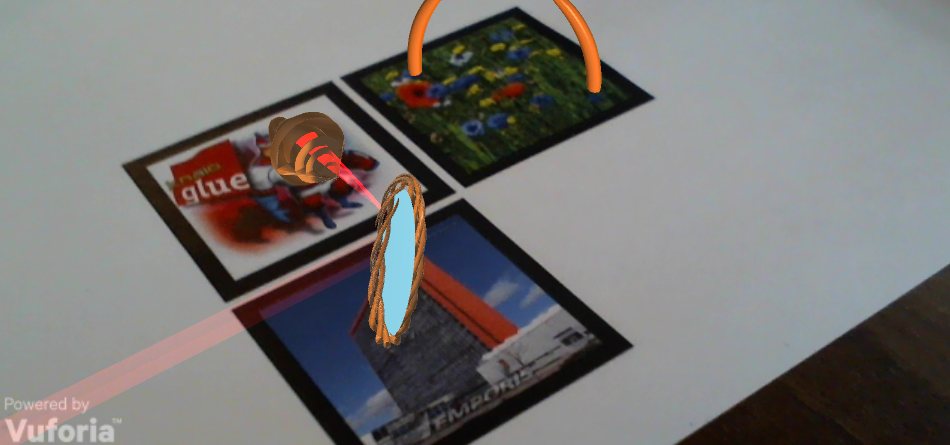
\includegraphics[width=\textwidth]{ResearchReport/demo.png}
\end{figure}
